\chapter{Method}
\section{Research Design}

\section{Content Analysis}
Having obtained seventy-seven retrospectives spanning over five years, the means of analyzing them had to be determined. 

The retrospectives consisted of five different sections being: Where and What, Actions, Comments, Signatures and Case Proceedings, as can be seen in \autoref{table:retrospective-format}. 
The ``Where and What'' section contained general data about the retrospective such as the date, iteration dates, iteration number, contact person and other general information. ``Actions'' described the improvement actions that had resulted from the retrospective. It contained a description for each action, who is responsible for that action, deadline, status and comments from the participants. The ``Comments'' section contained comments, if any, from the participants of the retrospective if they had any specific input for the retrospective in general. ``Signatures'' contained the signature for each participant in the retrospective. The last section,``Case Proceedings'' contained information about the changes in the document and circulation of it.

\begin{table}[!h]
	\begin{center}
	\caption{The section of the retrospectives}
	\label{table:retrospective-format}
	\makebox[\textwidth]{%
		\begin{tabular}{l | p{0.7\textwidth}}
		\hline
		Part & Description \\
		\hline
		Where and What & Containing general data about the retrospective such as date, iteration location, etc. \\
		Actions & Describes the actions resulting from the retrospective it also includes data on responsible person, deadline etc. \\
		Comments & General comments from the participants for the retrospectives. \\
		Signatures & The signatures from each participant participating in the retrospective. \\
		Case Proceedings & The changelog and circulation of the retrospective. \\
		\hline
		\end{tabular}
	}
\end{center}
\end{table}

While getting familiar with the retrospectives we found that the only section containing any value in the terms of organizational learning was the actions described in the ``Action'' section. In most of the retrospective multiple actions where described relating to different issues observed during the iteration. The format of the actions can be seen in \autoref{table:action-format}. 

\begin{table}[!h]
	\begin{center}
	\caption{An generic example of an action provided in the retrospectives.}
	\label{table:action-format}
	\makebox[\textwidth]{%
		\begin{tabular}{| l  p{0.5\textwidth} |}
		\hline
		Action x &  \\
		Deadline & 01.01.2015 \\
		Action description & Always add a week to the iterations during holidays. \\
		Comments & Resources are not reliable during holidays. \\
		Responsible unit & Team X \\
		User responsible for action & John Smith \\
		Status & Completed or In Process \\
		Completed & 31.01.2014 \\
		Type & Preventive or Corrective \\
		\hline
		\end{tabular}
	}
\end{center}
\end{table}

To retrieve any research-worthy knowledge from the many actions given by the retrospectives we wanted to make the actions comparable. We settled on tabulations as our analysis method of the actions. 

Tabulations provide easy means of rendering data comprehensible. Krippendorff ~\cite{Krippendorff2004} describes tabulations as: 

\begin{quote}
Tabulation refers to collecting same or similar recording units in categories and presenting counts of how many instances are found in each. Tabulations produce tables of absolute frequencies, such as the number of words in each category occurring in a body of text, or of relative frequencies, such as percentages expressed relative to the sample size, proportions of a total, or probabilities.
\end{quote}

For our case we are going use absolute frequencies to count the occurrences of different categories described in \autoref{method:categories}. Using relative frequencies would not suffice in our case where determining whether an action is twenty percent technical and eighty percent procedural or thirty percent technical and seventy percent procedural would be immensely difficult and not to mention impractical. Rather an action could be neither technical or procedural,be one of them, or be both. Thus resulting in us using absolute frequencies when we are counting occurrences of the different categories.

\subsection{Pilot Analysis}
Settling on tabulations as our means of content analysis the different categories had to determined. We performed a pilot study.
The pilot study was conducted in order to investigate the potential of analyzing a set of the 77 retrospective reports.  The pilot study was limited to 11 reports, where we picked every 7th retrospective chronologically. This distribution was chosen in order to get an even spread to represent the whole set, as well as keep the size manageable for the short preliminary study.

The pilot study analysis lasted for one week, and included agreeing on the parameters and methods for the study, as well as a short workshop session where the results were presented in front of a group of fellow researchers. This workshop session consisted of a short presentation of the findings of the study. After the presentation we had a brainstorming session where we received feedback on potential improvements, as well as general impressions. 

\begin{figure}[!h]
	\centering
	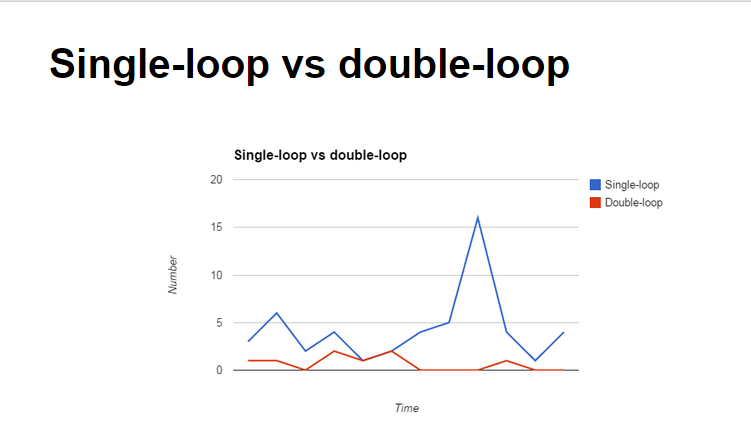
\includegraphics[width=\textwidth]{figures/Pilot_loop.PNG}
	\caption{An example of a slide from the pilot study presentation }
	\label{figure:Pilot Slide}
\end{figure}

\subsection{Categories}\label{method:categories}
The results of our pilot analysis gave us an extended set of categories that we will now describe further. Mainly we found six main themes that we could derive categories from. The six themes were: Nature, Context, Decision Making, Organizational Learning, Development and Management. We will describe each of these themes and their set of categories further in the sections below. A complete list is shown in \autoref{table:content-analysis-categories}. 

\begin{table}[h]
	\begin{center}
		\caption{The final set of themes and categories that the content analysis is based upon.}
		\label{table:content-analysis-categories}
		\begin{adjustbox}{width=\textwidth, totalheight=0.9\textheight, keepaspectratio}
			\begin{tabular}{| l | l | p{0.5\textwidth} |}
			\hline
			Theme & Category & Short Description  \\
			\hline
			Nature & Positive & If an action is a result of a continuation of a process \\ \cline{2-3}
			& Negative & Action is a result of a arisen problem \\ \cline{2-3}
			& Undefined & The nature of the action is unclear or undefined \\ \hline
			Context & Technical & If the action is related to some technical context. \\ \cline{2-3}
			& Process & Action is related to a process context \\ \cline{2-3}
			& Undefined & The action could not be related to either technical or process \\ 
			\hline
			Decision Making & Strategic & Action is suggesting long-term change \\ \cline{2-3}
			& Tactical & The action is related to identification and use of resources. \\ \cline{2-3}
			& Operational & If the action is ensuring effectiveness and day-to-day operations \\ \cline{2-3}
			& Undefined & If the action is unclear and doesn't fit any of the other decision making categories. \\ 
			\hline 
			Organizational learning & Single-loop & If the action do a change that only influence the effects \\ \cline{2-3}
			& Double-loop & If one understand the factors that influence effects, and the nature of this influence. \\ \cline{2-3}
			& Undefined & If the action unclear in terms of organizational learning \\ \hline
			Development Phase & Development & Action is related to the development phase \\ \cline{2-3}
			& Testing & The action is related to testing \\ \cline{2-3}
			& Documentation & Action is related to Documentation \\ \cline{2-3}
			& Builds & The action is related to building of software systems \\ \cline{2-3}
			& Release & The action is related to releasing of software \\ \cline{2-3}
			& Business & The action is related to business development \\ \cline{2-3}
			& Undefined & The action is not related to any of the development phases described above \\ 
			\hline
			Collaboration & Communication & Related to communication within a team \\ \cline{2-3}
			& Leadership & Action is related to leadership \\ \cline{2-3}
			& Competence & Action is a result of lacking knowledge or experience \\ \cline{2-3}
			& External relations & The action is related to customer relations or other external stakeholders \\ \cline{2-3}
			& Planning & The action is a result of bad or good planning \\ \cline{2-3}
			& Undefined & Action is not related to any of the collaboration issues \\
			\hline
			\end{tabular}
		\end{adjustbox}
	\end{center}
\end{table}
\afterpage{\clearpage}

\subsubsection{Nature}
The nature of the action is the first theme that the content analysis is going to inspect. We define the nature of the action as how the origins of the action began. Did they come from a problem that occurred during the iteration or is it a continuation of something that has been working well in the past. Through our analysis we will try to understand the origins of the actions and classify them either as positive, negative or undefined. We define our classifications below. 
\paragraph{Positive} Positive actions is those actions where the origins of the action is in a positive context. If the action represents a current good working practice being continued, or something uncommon happened that gave positive results, it would be classified as positive.
\paragraph{Negative} The negative actions are those actions that has its origins from a problem or abnormal issue resulting in negative results. If an action is a result of a problem or abnormal issue it is classified as an negative action. 
\paragraph{Undefined} In the cases where it is unclear whether the origins of the action is positive or negative we classify the action as undefined. Such occurrences can be a result of missing context or actions that seem to have neither positive issues or negative issues as its origin. 
\subsubsection{Context}\label{method:context}
The context surrounding the action will be analyzed. The context off the action is based on the underlying issue that leads to the needed action. We divide the issues into three main categories, technical, process and undefined. 
\paragraph{Technical}
A technical issue can be a issue relating to technical competence, bugs or problems.
\paragraph{Process}
A process issue stems from a problem with a process, or potential for improvements in the existing processes. This can for example relate to communication between colleagues or work scheduling.
\paragraph{Undefined}
 An undefined issue might not have any clear origin, or might be too loosely described to be classified easily.
\subsubsection{Decision Making}
Rational decision making is how decision makers should think and should act based on coherence and rationality, according to M. Drury et al. ~\cite{Drury2012}. N.B. Moe et al. ~\cite{Moe2011} appends bounded rational decision-making as the means of understanding how decision making is made in non-routine activities. N.B. Moe et al. reasons that both are needed when analyzing decision-making in an agile context:
\begin{quote}
Software development involves both routine and non-routine activities. Hence, it makes sense to use both rational and bounded rational decision making theories when explaining decisions in software development processes. 
\end{quote}
Drury et al. distinguishes between two types of decisions being made in an organization, the strategic and the tactical. Moe et al. distinguishes between three types: Strategic, tactical and operational. We will use the three-type model. Each decision type will be described in the following paragraphs. 
\paragraph{Strategic}
A strategic decision is a wide ranging decision dealing with multiple or sizable issues, often causing major changes and have a long term impact.Moe et al. describes the strategic decisions as the following: 
\begin{quote}
Strategic decisions are related to organizational goals and objectives. The information concerning such decisions is usually incomplete and the decision-making process may extend over a considerable period of time.
\end{quote}
The actions that are categorized as strategical is the ones that proposes changes that have a long term impact or proposes changes that are related to the organizational goals. 
\paragraph{Tactical}
A tactical decision is smaller than a strategic decision it seeks to deal with the distribution and use of resources available to the team. Moe et al. described it as: 
\begin{quote}
Tactical decisions are related to identification and use of resources.
\end{quote}
All actions that specifically proposes to identification of resources or proposes changes to how resources are spent will be classified as tactical.
\paragraph{Operational}
Moe et al. describes an operational decision as: 
\begin{quote}
Operational decisions deal with ensuring effectiveness of day-to-day operations within the organization. 
\end{quote}
Every action that are restricted to only day-to-day operations will be classified as operational decisions. They might be quick fixes that solve a single problem. 
\paragraph{Undefined}
An undefined decision might be difficult to categorize because of a lack of context or an unclear description.

\subsubsection{Organizational Learning}
Organizational learning is a process where an organization takes steps to improve its current work environments by reacting to issues that arise. These steps can be varied, and we divide them into single-loop, double-loop and undefined. Retrospectives have a central role in 	organizational learning, as described by Dingsøyr ~\cite{Dingsoyr2007}
\paragraph{Single-loop}
A single-loop action is an action designed to change or tune a process in order to improve it. The action does not seek to address underlying problems, and are a single-feedback loop from observing an issue to making a change. A retrospective can facilitate single-loop learning where the project team uses the input during the retrospective to make adjustments to their current work ~\cite{Dingsoyr2004}
\paragraph{Double-loop}
A double-loop action is designed to solve an issue, as well as address the underlying cause of the issue. This requires an understanding of the underlying issue and the nature of its influence. Double-loop decisions can be facilitated through a retrospective, often these are as a result of a more drastic need for change and an understanding of the underlying problem. ~\cite{Dingsoyr2004}

\paragraph{Undefined}
An action might not be clearly described, or the nature of the action can not be interpreted. We will classify these actions as undefined.

\subsubsection{Development}
An issue that is related to the development of the product is included in this category. The development process is the actual work performed to create the product, as well as processes directly related to this work. The different categories included in development were chosen after discussing with advisors, as well as personal experience from the writers
\paragraph{Development}
Development includes the writing of code, specifying requirements, construction the system architecture and other aspects of designing of the system. 
\paragraph{Planning}
An action that is categorized as planning is when the action is suggesting changes to planning in future iterations or is a result of an issue occurring in a former iteration. Estimations, task-prioritization, scheduling and etc. all goes under the planning category.
\paragraph{Testing}
Issues related to the testing of a product, this includes unit, module and system testing. Issues related to testing can also be communication between testers and developers.
\paragraph{Documentation}
Action that are categorized as documentation is those that are related to the documentation part of developing a system. Typical actions are those that describe or propose changes to documentation practices. This can also include tutorials that explains the product and improves usability. 
\paragraph{Builds}
During development of a software system building the software system can be a tiresome task. The actions that are categorized as builds are those who proposes practices that changes the current build practices.
\paragraph{Release}
When a system feature or a part of a system is finished, usually at the end of an iteration, one deploy the new part of the system into production, available for the users. For the actions that categorized as release, the action describe some aspect of the release practice and either proposes changes or suggest new practices.
\paragraph{Business}
Business development is a critical part for an organization to create profit. Software system often can save costs and create new business opportunities and as a part of a software development team one also has to consider business perspectives. We categorize all actions that are related to business development or proposes some business related changes as business. 
\paragraph{Undefined} If an action is neither of the development phases described above we classify it as undefined. 
\subsubsection{Collaboration}
One of the aspects during a software developing process is collaboration. Fægri ~\cite{Faegri2012} describes collaboration as the following: 
\begin{quote}
Collaboration is a key aspect of software development. Collaboration allows groups of software practitioners to deal with uncertainty, complexity and interdependence. And in dealing with these challenges, the group demonstrates its collective problem-solving ability.
\end{quote}
Through our pilot analysis we registered several activities that are related to collaboration. Communication, leadership, competence, external relations and planning all belongs beneath the collaboration banner, and we describe in detail how we classify each of them below. 
\paragraph{Communication}
Communication is a widely used word and concept, but it rarely is defined. By using Merriam-Webster dictionary ~\cite{MerriamWebster2015} we found a definition that can serve as a clarification: 
\begin{quote}
The act or process of using words, sounds, signs, or behaviors to express or exchange information or to express your ideas, thoughts, feelings, etc., to someone else.
\end{quote}
Nakakoji et al. ~\cite{Nakakoji2010} distinguishes between two types of communication related to software development, coordination communication and expertise communication. The first one being the process of coordinating the development activities and the last one being when a developer obtain some information regarding a software artifact, either through code comments, wikis or other means. 
We are however not going to distinguish between these two communication types in our content analysis as we believe the two differentiations is covered by the context of the action as described in \autoref{method:context}. For our content analysis we are simply going to count every instance of communication for every action that is related to communication between team-members regardless if it is through text, speech or other means of communication.
\paragraph{Leadership}
As is the case with communication, leadership is also widely used concept, that is rarely specified. Again we turn to Merriam-Webster \cite{MerriamWebster2015} for a definition: 
\begin{quote}
The power or ability to lead other people.
\end{quote}
Agile development teams is often self-organized as it is one of the principles in the agile manifesto \cite{AgileManifesto2015}. This can result in no clear leadership. For our content analysis we are going to consider decisions and guidelines set by the group itself as leadership activities. We categorize actions as leadership if they somehow suggests changes to leadership or if the actions is a result of some leadership related issue. 
\paragraph{Competence}
We define competence as the ability to perform a certain task in a adequate quality. Each member within an agile team has their own set of knowledge that they use to solve different tasks. If any issues arises and the group is lacking the knowledge to counter it we categorize the action created to resolve it as an competence action. An example could be issue of lacking the knowledge resolving a database error and the action is to send one developer at a database course. This action would then be categorized as an competence action.
\paragraph{External Relations}
By the category external relations we mean if the team has any actions that is a result of issues arising from external factors or the actions that team is creating to inflict some external factors. Example of external relations can be customer relations, communication with server maintenance team or other development teams.   
\paragraph{Undefined}
For those actions that the origin is unclear and the goal is not related to any of the collaboration categories we categorize them as undefined.

\subsection{Reoccurring issues}
A retrospective is intended to highlight issues and potential actions that can be taken to correct or improve the issues. However it is not necessarily the case that every action is implemented as intended, or in the time frame originally intended. As such issues might come up again and again. Being able to identify these long term issues and address them before they become reoccurring is a clear potential improvement for a team or organization. Therefore it is of great interest to identify these issues in our analysis. We will be looking through the available information and noting if an issue arises multiple times over time. Also of interest are unresolved issues, that is issues that are raised and a corrective action is agreed upon, but the action is either not implemented or implemented fully.

\subsection{Processing Steps}
To perform our content analysis we first defined a set of processing steps that both authors were to follow. All the processing steps can be seen in \autoref{table:content-analysis-steps}.

\begin{table}
	\begin{centering}
		\caption{Description of the content analysis steps.}
		\label{table:content-analysis-steps}
		\begin{tabular}{l p{0.8\textwidth}}
			Step & Description \\ 
			\hline
			1 & Specify and document all the tabulation categories. \\
			2 & Send analysis documentation to the case participants to get feedback on the analysis measurements. \\
			3 & Create a spreadsheet for each author containing data on all the categories and all the actions. \\
			4 & Each author read through all the retrospectives separately, setting marks for each category that an action fits in. \\
			5 & When both authors were finished reading through all the retrospective they compared the results and put everything into a combined spreadsheet. If the authors disagreed on their markings a short discussion would commence and one would try to find an agreement. If an agreement could not be found the authors would turn to other external researchers to help identify the correct solution. \\
			6 & The content analysis was finished when all the actions were in the combined spreadsheet. \\
		\end{tabular}
	\end{centering}
\end{table}

The first step was to specify all the tabulation categories that were going to be included in the content analysis. Once all the categories was found and specified we documented them to ensure both authors had the same understanding of what each category meant. 

When the categories had been documented we sent them to the case participants to get feedback on the analysis measurements and verify that it were not anything that we had overlooked that the participants would like answers to. 

Once the feedback was incorporated into the content analysis we created a spreadsheet containing all the actions along the top row and all the categories along the first column. \todo[inline]{Reference to figure or appendix the spreadsheet model or full spreadsheet} We created one spreadsheet for each author and one extra that would later be used for comparison. 

When the spreadsheets were done the next step was analyzing all the actions. Each author, separately, read through all the retrospectives and for each action marked which categories it belonged to. Each action could belong to several categories for an example an action could belong to both Testing and Documentation. For each of the six themes at least one mark had to be put down, and the maximum marks would be the number of categories in that theme. 

After all the retrospectives were read through and every action was tabulated the authors compared their results. For each action the authors would compare all the marks set for that action and if they both agreed upon all the mark the action would be copied to a new spreadsheet. If the authors disagreed they would go back to the action read it once more and try to find a classification that both could agree to. If this turned impossible we would seek advice from external researchers to gain a suitable solution. 

Once all the actions were compared and all the actions was in the new spreadsheet the content analysis was finished and data could then later be extracted from the spreadsheets. 

\subsection{Content Analysis Limitations}
In this section we will describe the challenges and limitations of our content analysis from the 77 retrospectives. Mainly there were two challenges that occurred during our content analysis, missing contexts and borderline actions. Each is described in detail below. 
\subsubsection{Missing Contexts}
As the retrospectives we were given mostly contained actions that resulted from the retrospective meetings, context of how the actions were brought to light could sometimes be missing. In those cases the actions either could have come from a problem happening during the iteration, a new idea that were put forth during the iteration or something similar. As some of the actions lacked context we included the undefined category to each theme so that in the cases were we could not tell whether an action was in a concrete development phase, or another theme, we could put it in undefined. 
\subsubsection{Borderline Actions}
Borderline actions was the second challenge while performing our content analysis. An example is the action: 
\begin{quote}
To improve the understanding of the processes, the workflow diagrams and the other relevant documentation should be copied to the WIKI.
\end{quote}
This action could either be understood as ``The workflow diagrams and other relevant documentation is so good that we should put it on the WIKI'' or ``People do not have enough understanding of the processes and we should give them more documentation''. The first option could be classified as an positive action as the working documentation is good and should be used better, while the second option would be classified as a negative action as it is a problem that the understanding of the processes are not good enough. This action would be classified as undefined in our analysis as it both require more context and as it lacks the context can be a borderline action between positive and negative. 

To deal with the borderline actions we added the steps of each author doing a separate analysis before comparing with the other author to identify the borderlines and find a adequate classification for them.


\section{Visiting team: Feedback session and interview}
As the final part of the first analysis we visited the team we had analyzed, and hold a feedback session, where we would gather valuable input from the team and their reflections on the analysis. This visit was planned in advance and we would have a one hour presentation, followed by a discussion, then there would be a lunch. After the lunch the team members would be free to be interviewed. An interview with the SCRUM master had already been scheduled in advance.

\subsection{Feedback session}
The presentation was held in a meeting room in front of the team. The concept of the analysis was first explained and discussed with the team members, in order to ensure that there existed a common understanding of the work being presented. The presentation was also simultaneously a dialog between the presenters and the team. This was facilitated by constantly asking questions and encouraging discussion. One of the ways of encouraging discussion was to ask the team ``What expectations do you have for this category?'' before showing the results of the analysis. This ensured that we got their speculation as well as their reaction to the analysis. 

\subsection{Interview with SCRUM master}
After the lunch we had an interview with the SCRUM master of the team. We spent a short while preparing and reviewing the questions we had prepared. The interview would be held in a semi-structured manner with the goal of having an open discussion of the results of the feedback session as well as gaining insight on the themes of the thesis. During the interview notes were taken, as well as recorded, and the SCRUM master was encouraged to speak his mind on relevant subjects. 

\section{Interviews}
After the analysis of the retrospectives we performed a second data collection, using interviews of retrospective practitioners. We decided on a semi-structured interview, in order to be free to improvise as well as being prepared to ask stimulating questions to the interview subject.

\subsection{Semi-structured interviews}
We decided to use a semi-structured interview as our model for the interviews. An unstructured, or semi-structured does not have a complete script, and leaves room for improvisation, unlike a structured interview where there is a complete script. \cite{Myers2007} This approach was chosen to leave the interview subject free the elaborate on subjects they found interesting. 

A list of questions was prepared in order to serve as a guideline for the interview. This interview guide was divided into five sections relevant for our research being: ``General overview'', ``Team dynamics'', ``Organizational learning'', ``Team specific questions'' and ``Anything else''. A short description of each of these are shown in \autoref{table:interview-guide-overview}. The complete interview guide including all the questions can be found in \todo[inline]{appendix link til guide}

\begin{table}
	\begin{centering}
	\caption{Interview guide overview}
	\label{table:interview-guide-overview}
	\begin{tabular}{l p{0.8\textwidth}}
	 	Step & Description \\ 
		\hline
		General overview & Questions relating to the holding of the retrospective and learning\\
		Team dynamics & Questions on how team dynamics are handled and how they are experienced in the team \\
		Organization learning & Questions on how the team approach learning \\
		Team specific questions & Questions crafted through preparing specifically for the team in question \\
		Anything else & Summary questions intended to cover potentially missed topics \\
	\end{tabular}
	\end{centering}
\end{table}

In order to conduct a successful semi-structured interview Myers and and Newman mentions several factors that need to be acknowledged. \cite{Myers2007} Among these are the lack of trust, elite bias and ambiguity of language. In order to avoid these potential pitfalls we spent time ensuring a mutual understanding and respect with the interview subject, for example by explaining our intentions and maintaining a friendly tone during the interview. 

\subsection{Interview Subjects}
\todo[inline]{Write about the interview subject selection}